\subsection{Exercise 7.1: Sorting by Polar Angle}
\textbf{Problem:} The polar angle of a point $p_i$ with respect to an origin $p_0$ is the angle from the semi-horizontal straight line $r$ and the vector $\overrightarrow{p_0p_i}$. The positive direction of the angle is counterclockwise. Angles are in the interval $[0, 2\pi)$. Write pseudocode to order $n$ points $q_1, \ldots, q_n$ by their polar angles in increasing order, with $O(n \log n)$ running time.

\textbf{Solution Strategy:}
\begin{enumerate}[noitemsep]
    \item Let $p_0 = [x_0, y_0]$ and $q_i = [x_i, y_i]$.
    \item Divide points $A = \{q_1, \ldots, q_n\}$ into:
        \begin{itemize}[noitemsep]
            \item $A_1$: Points with $y \geq y_0$
            \item $A_2$: Points with $y < y_0$
        \end{itemize}
    \item Polar angles in $A_1$ are in $[0, \pi]$, in $A_2$ are in $(\pi, 2\pi)$.
    \item Use ANGLEMEREGE-SORT to sort both $A_1$ and $A_2$.
\end{enumerate}

\textbf{Algorithm Details:}
\begin{itemize}[noitemsep]
    \item PARTITIONANGLE:
        \begin{itemize}[noitemsep]
            \item Purpose: Divides the array into two groups based on the y-coordinate relative to $y_0$.
            \item Process: Iterates through the array, swapping elements to ensure points in $A_1$ have polar angles in $[0, \pi]$ and points in $A_2$ in $(\pi, 2\pi)$.
            \item Complexity: $O(n)$, as each point is processed once.
        \end{itemize}
    \item ANGLEMERGE-SORT:
        \begin{itemize}[noitemsep]
            \item Purpose: Sorts points within each subset based on polar angles.
            \item Process: Uses a modified merge sort where the cross product is used to compare angles, ensuring correct order.
            \item Complexity: $O(n \log n)$, typical for merge sort algorithms.
        \end{itemize}
    \item ANGLE-SORT:
        \begin{itemize}[noitemsep]
            \item Purpose: Integrates the above methods to sort the entire set $A$.
            \item Process: Calls PARTITIONANGLE to separate the points, then applies ANGLEMEREGE-SORT to each subset.
            \item Complexity: $O(n \log n)$, combining the efficiencies of partitioning and sorting.
        \end{itemize}
\end{itemize}

\textbf{Pseudocode:}
\begin{verbatim}
procedure PARTITIONANGLE(A, y0):
    i = 0
    for j = 1 to n do
        if y.A[j] >= y0 then
            i = i + 1
            exchange A[i] with A[j]
    return i + 1

procedure ANGLEMEREGE-SORT(A, p, r):
    if p < r then
        q = (p + r) / 2
        ANGLEMEREGE-SORT(A, p, q)
        ANGLEMEREGE-SORT(A, q + 1, r)
        ANGLEMEREGE(A, p, q, r)

procedure ANGLE-SORT(A):
    if A != NIL then
        n = length.A
        q = PARTITIONANGLE(A, x0)
        ANGLEMEREGE-SORT(A, 1, q - 1)
        ANGLEMEREGE-SORT(A, q, n)
\end{verbatim}

\textbf{Complexity Analysis:}
\begin{itemize}[noitemsep]
    \item PARTITIONANGLE: $O(n)$
    \item ANGLEMEREGE-SORT: $O(n \log n)$
    \item Overall complexity: $O(n \log n)$
\end{itemize}

\textbf{Key Insights:}
\begin{itemize}[noitemsep]
    \item Sorting by polar angle requires careful handling of angle wrap-around.
    \item Efficient sorting is crucial for applications in computational geometry.
    \item Polar angles can be computed using $\text{atan2}(y_i - y_0, x_i - x_0)$.
\end{itemize}

\subsection{Exercise 7.3: ANY-SEGMENTS-INTERSECT}
\textbf{Problem:} Argue that \texttt{ANY-SEGMENTS-INTERSECT} works correctly even if three or more segments intersect at the same point.

\begin{center}
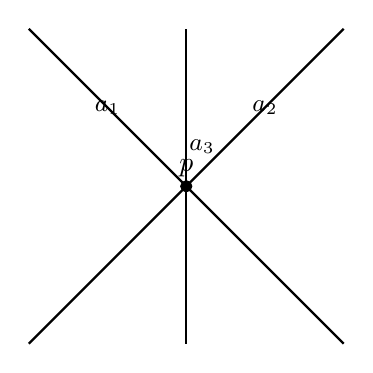
\begin{tikzpicture}
    \draw[thick] (0,0) -- (4,4);
    \draw[thick] (0,4) -- (4,0);
    \draw[thick] (2,0) -- (2,4);
    \node at (1,3) {\small $a_1$};
    \node at (3,3) {\small $a_2$};
    \node at (2.2,2.5) {\small $a_3$};
    \filldraw[black] (2,2) circle (2pt) node[anchor=south] {$p$};
\end{tikzpicture}
\end{center}

\textbf{Solution Strategy:}
\begin{enumerate}[noitemsep]
    \item Identify the conditions under which \texttt{ANY-SEGMENTS-INTERSECT} returns true.
    \item Analyze the behavior of the algorithm when three or more segments intersect.
    \item Prove correctness by considering event points and the sweep line.
\end{enumerate}

\textbf{Algorithm Details:}
\begin{itemize}[noitemsep]
    \item \textbf{Intersection Detection:}
        \begin{itemize}[noitemsep]
            \item Inserts a segment when it intersects with the above or below segment.
            \item Deletes a segment when its adjacent segments meet at a point.
        \end{itemize}
    \item \textbf{Event Point Analysis:}
        \begin{itemize}[noitemsep]
            \item Considers the first intersection point $p$ of $n$ segments.
            \item Analyzes the left and right points of segments at $p$.
        \end{itemize}
\end{itemize}

\textbf{Pseudocode Explanation:}
The pseudocode iterates through each event point, which represents either the start or end of a segment. When a left endpoint is encountered, the segment is added to the active set. If a right endpoint is reached, the segment is removed. The algorithm checks for intersections by evaluating if three or more segments meet at a point, returning true if so.

\textbf{Complexity Analysis:}
\begin{itemize}[noitemsep]
    \item Event processing: $O(n \log n)$
    \item Intersection checks: Efficient for multiple segments
\end{itemize}

\textbf{Key Insights:}
\begin{itemize}[noitemsep]
    \item The algorithm correctly identifies intersections involving multiple segments.
    \item The sweep line approach efficiently handles complex intersections.
\end{itemize}

\subsection{Exercise 7.4: ANY-SEGMENTS-INTERSECT with Vertical Segments}
\textbf{Problem:} Show that \texttt{ANY-SEGMENTS-INTERSECT} works correctly in the presence of vertical segments if we treat the bottom endpoint of a vertical segment as if it were a left endpoint and the top endpoint as if it were a right endpoint. How does your answer to Exercise 3 change if we allow vertical segments?

\begin{center}
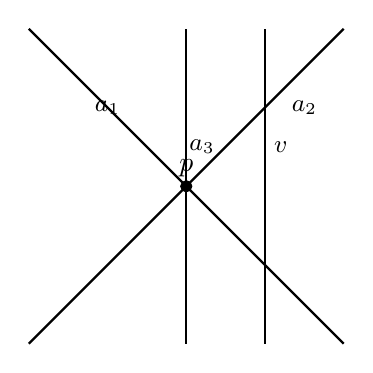
\begin{tikzpicture}
    \draw[thick] (0,0) -- (4,4);
    \draw[thick] (0,4) -- (4,0);
    \draw[thick] (2,0) -- (2,4);
    \draw[thick] (3,0) -- (3,4);
    \node at (1,3) {\small $a_1$};
    \node at (3.5,3) {\small $a_2$};
    \node at (2.2,2.5) {\small $a_3$};
    \node at (3.2,2.5) {\small $v$};
    \filldraw[black] (2,2) circle (2pt) node[anchor=south] {$p$};
\end{tikzpicture}
\end{center}

\textbf{Solution Strategy:}
\begin{enumerate}[noitemsep]
    \item Treat vertical segments with special rules for endpoints.
    \item Analyze how vertical segments affect the intersection detection.
    \item Prove correctness by considering vertical and non-vertical interactions.
\end{enumerate}

\textbf{Algorithm Details:}
\begin{itemize}[noitemsep]
    \item \textbf{Vertical Segment Handling:}
        \begin{itemize}[noitemsep]
            \item Treat the bottom endpoint as a left endpoint.
            \item Treat the top endpoint as a right endpoint.
        \end{itemize}
    \item \textbf{Intersection Detection:}
        \begin{itemize}[noitemsep]
            \item Check intersections with vertical segments using the sweep line.
            \item Ensure correct ordering of event points.
        \end{itemize}
\end{itemize}

\textbf{Pseudocode Explanation:}
The pseudocode processes each event point, treating vertical segment endpoints according to their roles. By treating the bottom as a left endpoint and the top as a right endpoint, the algorithm maintains the correct order and checks for intersections. This adjustment ensures that vertical segments are handled without altering the fundamental logic of the sweep line approach.

**Impact of Vertical Segments:** Allowing vertical segments in Exercise 7.3 would require treating their endpoints as described, ensuring that intersections involving vertical segments are detected correctly. The algorithm's logic remains intact, with the addition of handling vertical segment endpoints appropriately.

\textbf{Complexity Analysis:}
\begin{itemize}[noitemsep]
    \item Event processing: $O(n \log n)$
    \item Intersection checks: Efficient for vertical and non-vertical segments
\end{itemize}

\textbf{Key Insights:}
\begin{itemize}[noitemsep]
    \item The algorithm handles vertical segments by adjusting endpoint roles.
    \item The sweep line approach remains effective for complex intersections.
\end{itemize}
